% Chapter 7

\begin{savequote}[\quotewidth]

\qauthor{Shark}
\end{savequote}

\chapter{SFC×GC for the determination of FAMEs and PAHs in diesel fuel.} % Main chapter title
\label{Chapter7} % For referencing this chapter elsewhere, use \ref{Chapter7}

\section{Introduction}

In South Africa the quality of biodiesel is regulated by the technical standard
SANS 1935, and petrodiesel by SANS 342. There is a considerable overlap in the
requirements of the two, as discussed in Section \ref{sec:Comparison},
illustrated in Figure \ref{fig:Venn}. Two of the requirements of SANS 342 that
does not overlap with SANS 1935 are the allowed amounts of polycyclic aromatic
hydrocarbons (PAHs) and fatty acid methyl esters (FAMEs). This chapter's
discussion introduces the application of SFC×GC to these determinations. 

\subsection{FAMEs in diesel}

Biodiesel can be blended in all proportions with diesel obtained from petroleum
(\keyword{petrodiesel}). To reduce the carbon footprint of diesel fuel,
legislators are encouraging the use of blended fuels. In South Africa standard
grades of diesel may contain up to \SI{5}{\percent} volume fraction biodiesel, 
and higher fractions of FAMEs are allowed as different grades. Manufacturers might
also add biodiesel to their fuel formulations to present improve properties such as
lubricity \autocite{Knothe2005}, or to reduce emissions \autocite{Wattrus2016}.

The prescribed test method for FAMEs in standard diesel is EN 14078. This is an
infrared absorption method. This method measures the absorption of infrared
radiation at \SI{1745}{\per\centi\metre} (\SI{5.4}{\micro\metre}). This method
specifies a \SI{0.5}{\milli\metre} pathlength cell. The equivalent method
prescribed by ASTM D7371 specifies attenuated total reflection (ATR) sampling,
which simplifies sample handling but complicates calibration. Both these methods
makes some assumptions about the sample, and the methods suffers from inaccuracy
if those assumptions do not hold \autocite{Pinho2014}.

\subsection{PAHs in diesel} 

Polycyclic aromatic hydrocarbons (PAHs) are noxious pollutants and are therefore
regulated when possible. The primary source of PAHs in the environment is
combustion, of which a portion is in internal-combustion engines.  PAHs might
escape from diesel fuel during normal operations, or in accidents. Additionally,
the higher the proportion of aromatic compounds in diesel fuel, the higher the
PAH emissions of the engine that uses it. Therefore, the amount of PAHs in
diesel is regulated.

ASTM D5168 \autocite{ASTMD5186} is an SFC-FID method for determining the amount and type of aromatic
compounds.

\subsection{SFC×GC of petrodiesel/biodiesel blends}

\todo{k-primes}

\section{Experimental}

\subsection{Samples} 

A sample was prepared by blending \SI{7}{/percent} of biodiesel from canola
(labelled "rapeseed methyl ester" (RME)) with a commercial low-sulfur diesel. In a
GC×GC-MS analysis the relative percentages of total ion intensity for different
classes of compounds were \SI{68.19}{\percent} alkanes, \SI{18.10}{\percent}
alkenes, \SI{13.69}{\percent} aromatics and \SI{0.01}{\percent} oxygenates
\autocite{Smit2015}.

\todo{Spiked diesel sample}

\subsection{SFC}

The injection system described in Section
\ref{sec:SFCInjection} was used to inject a \SI{0.5}{\micro\litre} volume of
this undiluted \todo{7\%} blend.

The SFC used neat carbon dioxide at \SI{200}{\bar} inlet pressure as mobile
phase. The column consisted of five HPLC bare silica columns
(\SI{150}{\milli\metre} $\times$ \SI{4.6}{\milli\metre}, 3 $\mu$m particles)
(Restek, Pinnacle DB Silica) connected in series.

\subsection{Modulation}

\todo{Check modulation details}

The SFC eluate fractions of \SI{2}{\second} were collected on the GC column
cooled to a temperature of \SI{-20}{\celsius}. The inlet vent was held closed
for \SI{4}{\second}, and then opened for \SI{1}{\second} to release excess
pressure.

\todo{Talk about }
\todo{Add vent time increase}

\subsection{GC}

\todo{Correct column (HP DB5 equvalent)}
The column used in the fast gas chromatograph was an OV-5 column, which has a
stationary phase comprised of \SI{5}{\percent} diphenyl, \SI{95}{\percent}
dimethylpolysiloxane. It was \SI{1}{\metre} long, with an internal diameter of
\SI{0.25}{\milli\metre}. The thickness of the stationary phase was
\SI{0.25}{\micro\metre}.

\todo{Check temperature ramp}
The temperature was ramped from \SI{-20}{\celsius} at a rate of
\SI{1800}{\celsius\per\minute} to \SI{250}{\celsius}, where it was maintained
for \SI{6}{s}. After the temperature program had ended the column was cooled to
\SI{-20}{\celsius} again and the next fraction was collected.

The detector was an FID at \SI{350}{\celsius}. The FID response was recorded,
and so a total of \todo{370} fast GC chromatograms were collected to compile the 2D
chromatogram.

\section{Results}

Figure \ref{fig:PAH_FAMEs} shows the SFC×GC chromatogram of the diesel/biodiesel blend.

\begin{figure}
	\centering
	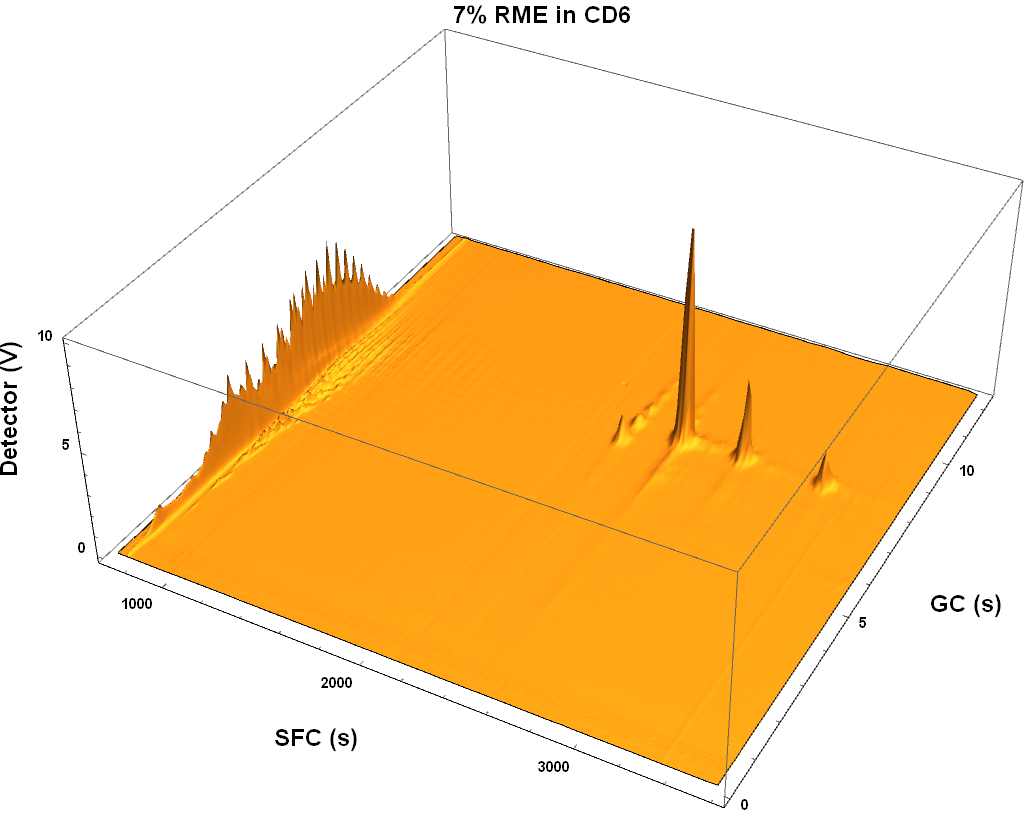
\includegraphics[width=\textwidth]{Figures/PAH_FAMEs.png}
	\decoRule	
	
\caption[Biodiesel separated from petrodiesel.]{The separation of the biodiesel
and petrodiesel in a \SI{7}{\percent} blend. The hydrocarbons elute completely
before the first FAME elute, offer interference-free determination of both.}

	\label{fig:PAH_FAMEs} 
\end{figure}

\todo{Aromatics section}

\todo{Spiked diesel}

\section{Discussion}

\todo{Adjustable modulation}

\todo{Peak assignment}

\todo{Open vent}

The chromatogram of the biodiesel/petrodiesel blend (Figure \ref{fig:PAH_FAMEs}) shows
that the blend was separated into two distinct groups of compounds. At a \oneD
(SFC) retention time of about \SI{160}{\second} the hydrocarbons from the
petrodiesel part of the blend elutes. To those familiar with petrochemical
chromatography the characteristic unresolved complex mixture (``hydrocarbon
hump'') topped by alkane peaks will be instantly recognizable as representing
a petroleum product. (See Figure \ref{fig:HCHump} for an example.)


\begin{figure}
	\centering
	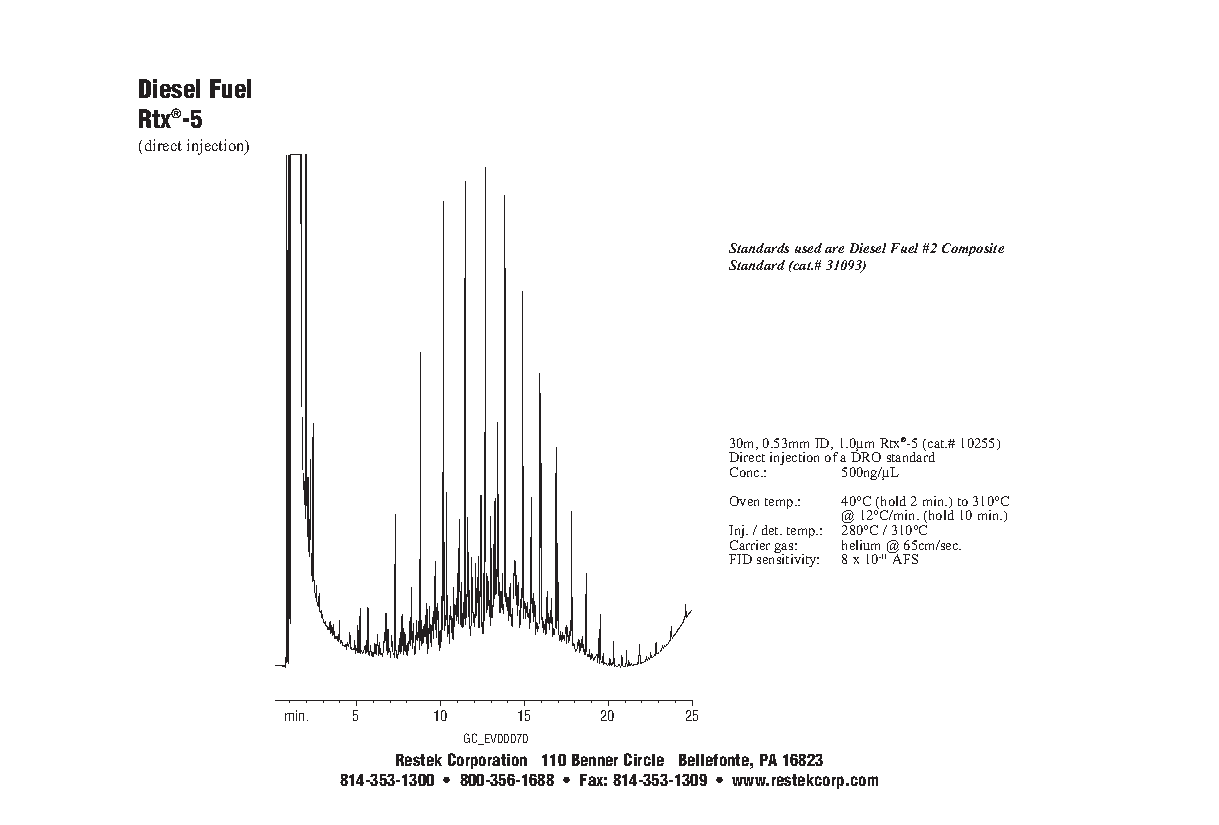
\includegraphics[width=\textwidth]{Figures/hchump.pdf}
	\decoRule	
	
\caption[An example of a petrochemical fuel chromatogram.]{An example of a GC
chromatogram obtained from a petroleum-based diesel fuel sample, showing the
unresolved complex mixture topped by alkane peaks.}
	
	\label{fig:HCHump} 
\end{figure}

Between the \textsuperscript{1}D retention times of \SI{300}{\second} and
\SI{480}{\second} the peaks of the FAMEs are seen, clearly separated by number
of double bonds in the SFC dimension, and by volatility in the GC dimension.
When compared to Figure \ref{fig:2DSunflower} \todo{the RME is indeed from Canola}.

This separation shows that SFC×GC can be used to investigate the biodiesel
component of petrodiesel/biodiesel blends without sample pre-treatment or
specialized columns. The intrinsic orthogonality provides easy identification of
components and the excess separation space allows for the addition of suitable
internal standards for reliable qualitative and quantitative analysis with the
robust FID with its predictable response. Expensive
mass spectrometric detection is unnecessary

Being able to determine the biodiesel content of biodiesel blends may prove
useful in at least two scenarios: 

The first is in monitoring blending. Biodiesel, essentially a mixture of esters,
is quite polar compared to petrodiesel, essentially a mixture of hydrocarbons.
This means that blending might not be a matter of just pumping the relevant volumes
of the respective fuels into a tank and relying on diffusion to complete the
mixing. Being able to determine the amount of biodiesel in different samples of
a blend will provide assurance that the blend is homogenous and should perform
according to expectations. While such a test is perhaps better performed using a
spectroscopic method, SFC×GC can provide information for calibration, and will
of course be invaluable during trouble shooting.  

The second application of SFC×GC is in regulating biodiesel content. In some
political environments fuels might be taxed according to their
biologically-derived content, for example to promote agriculture or to meet
carbon emissions targets. Sometimes biological content is not encouraged by
taxation, but simply mandated. Such incentives and mandates are of course liable
to corruption, and therefore the ability to monitor the blending of the fuels is
needed. The most reliable way to differentiate between organic matter derived
from biological sources and organic matter derived from fossil sources is a
radiochemical method, where the content of radioactive \textsuperscript{14}C is
determined. (Organic material from fossil sources contains no
\textsuperscript{14}C.) The technical standard ASTM D6866 provides an approved
method. But radiochemical methods require specialized equipment and trained
staff, whereas fuel laboratories more often have experience with chromatographic
techniques and might find SFC×GC a useful technique to provide evidence that a
diesel fuel blend contains the stated amount of biodiesel.


, and might provide a way to quantify the biodiesel component in blends
with petrodiesel, and cost-effective, accurate and reliable quantitation of the
biodiesel component in blends with petrodiesel can be expected.


\section{Conclusion}

\todos